\documentclass[11pt]{article}
\usepackage[margin=1in]{geometry}
\usepackage[T1]{fontenc}
\usepackage{lmodern}
\usepackage{amsmath,amssymb}
\usepackage{graphicx}
\usepackage{booktabs}
\usepackage{float}
\usepackage{xcolor}
\usepackage{enumitem}
\usepackage{caption}
\usepackage{tikz}
\usetikzlibrary{positioning,arrows.meta,shapes.geometric}
\usepackage[colorlinks=true,linkcolor=blue!50!black,urlcolor=blue!50!black,citecolor=blue!50!black]{hyperref}
\setlist{itemsep=2pt,topsep=4pt}
\emergencystretch=3em
\captionsetup{font=small,labelfont=bf}
\graphicspath{{figures/}}

\title{\textbf{An Agreement-Gated Relay-BP Decoder for the Gross Code}\\[4pt]
\large MidQWest 2026 Hackathon --- Infleqtion Challenge 1: ML-assisted decoding of the $[[144,12,12]]$ Gross code}
\author{Team Heisenbugs\\[2pt]\small Written with Claude (Anthropic), GPT (OpenAI, via Codex) and Gemini (Google, via Antigravity)}
\date{November 2026}

\begin{document}
\maketitle

\begin{abstract}
\noindent
We built a decoder for the $[[144,12,12]]$ Gross code that puts a cheap \emph{agreement gate} in front of
Relay-BP. A fast Relay-BP run decodes each syndrome. If it needs more than its deterministic first leg, a second, differently seeded
run checks it, and the answer is accepted only if both agree on the logical class. Disputed or unsolved shots go to a full Relay-BP ``referee''.
A noise detector estimates the physical error rate from the alarm count and chooses the gate's settings.
On identical simulated shots at the challenge's noise levels ($p = 0.003, 0.004, 0.005$) the gate has
\textbf{3--8$\times$ fewer logical failures than BP-OSD}. Its logical error rate shows no statistically significant difference from Relay-BP's (non-inferiority within 20\% is
shown at $p=0.005$; at $0.003$ and $0.004$ it is inconclusive), while it uses \textbf{13--61\% less mean decoding time}. Tail latency
improves at $p=0.003$ (p99 $0.73\times$) but not at $p=0.004$--$0.005$, where it is roughly equal to Relay-BP's. In this simulator, which
uses uniform noise, a small neural network estimates the noise level no better than counting alarms.
A learned pre-decode ``hard-shot spotter'' also gave no net gain. We report both negative results and point to in-flight
escalation decisions as the next place where machine learning could add measurable value.
\end{abstract}

\tableofcontents
\newpage

%=====================================================================
\section{The problem}

Quantum error correction protects quantum information by spreading it across many imperfect physical qubits. This protection requires a classical decoder: software that interprets repeated measurements and decides which errors most plausibly occurred. A useful decoder must make few logical mistakes and finish quickly. These objectives can conflict, because the measurements that are hardest to interpret may also require the most computation.

Our task comes from Challenge 1 of the MidQWest 2026 Infleqtion ``Qubits \& Gradients'' challenge. It asks for ML-assisted decoding of the $[[144,12,12]]$ Gross code, a quantum low-density parity-check code, or qLDPC code. The required comparison is against two supplied decoders, BP-OSD and Relay-BP, at physical noise strengths
$p \in \{0.003,0.004,0.005\}$.
The deliverables include logical error rates, decoding latency, resource comparisons, a GitHub repository, a plot, and a presentation.

The central question is whether we can spend less computation on easy cases while preserving accuracy on difficult ones. This is more demanding than making a decoder faster on average. An inexpensive decision to accept a wrong answer can damage error correction, while an unsuccessful fast attempt followed by a slow fallback can increase latency.

\subsection{What the decoder receives and predicts}

The challenge uses a simulated memory experiment. Quantum information is prepared, held through 12 noisy syndrome-measurement cycles, and finally read out without additional noise. There are separate experiments for $X$ memory and $Z$ memory, corresponding to preparation in $|+\rangle$ and $|0\rangle$, respectively.

For each basis, the decoder receives 936 binary detector outcomes. A detector is an alarm indicating an unexpected change in the measurement record. The decoder must explain those alarms using a model containing 8,784 possible error mechanisms. Its final prediction concerns the 12 logical observables stored by the code.

The supplied kit uses \texttt{stim} to construct and sample the noisy circuits. It provides circuits, detector-model matrices, sampling utilities, and baseline decoders. The full $XYZ$ decoding problem contains 1,728 detectors and approximately 68,000 mechanisms; the separate basis problems give the dimensions used above.

The challenge scores the two memory experiments jointly. Shot $k$ from the $X$ experiment is paired with shot $k$ from the $Z$ experiment. A pair fails if either decoder prediction gets any logical observable wrong. Thus, success means protecting the complete set of logical observables in both members of the pair.

\subsection{Why speed and accuracy must be measured together}

BP-OSD and Relay-BP provide different starting points. BP-OSD combines a fast iterative procedure with an algebraic search that supplies a syndrome-consistent answer. Relay-BP searches through multiple iterative trajectories and chooses among the solutions it finds. Relay-BP achieves strong accuracy, but its runtime varies considerably between shots.

The kit reference illustrates this tradeoff. At $p=0.004$, it reports logical error rates per cycle of $4.4 \times 10^{-3}$ for BP-OSD and $8.7 \times 10^{-4}$ for Relay-BP, using 10,000 shots per basis. Its reported mean decoding times are $0.33$ seconds and $0.38$ seconds, respectively, while Relay-BP's 99th-percentile latency is about 6 seconds. These are reference measurements, not universal timing constants.

Our initial approach was hierarchical: a light decoder handles easy shots, while harder shots receive additional computation. This leads naturally to an acceptance or escalation decision for each complete shot. A proposed router must therefore be judged by the logical failures and runtime of the complete decoding system. Its own classification accuracy is insufficient: different routing mistakes have very different consequences.

The acceptance decision also needs evidence beyond internal confidence. A decoder can find an explanation that matches every alarm yet predicts the wrong logical outcome. Much of the challenge is identifying when a fast answer is reliable enough to accept.

The bonus theme concerns qubit loss and heralding, but the supplied kit does not simulate loss. The experiments discussed here concern circuit-level depolarizing noise. This scope matters when interpreting both decoder performance and the value of machine learning.

\section{Prerequisites}

\subsection{Physical qubits, logical qubits, and stabilizer checks}

A physical qubit is an individual qubit used by the circuit. A logical qubit is information encoded collectively across physical qubits. Encoding introduces redundancy so that some physical errors can be detected and corrected without measuring the stored logical information directly.

The notation $[[n,k,d]]$ describes a quantum code with $n$ data qubits, $k$ logical qubits, and distance $d$. The Gross code is $[[144,12,12]]$: it stores 12 logical qubits in 144 data qubits and has distance 12. The experiment also uses 144 check qubits, giving 288 physical qubits in total.

The distance is the minimum weight of a nontrivial logical Pauli operator: an operation that changes the encoded information while escaping the code's stabilizer checks. Weight counts the data qubits on which that operator acts nontrivially. Distance is a property of the code; it is not a count of how many circuit faults a particular decoder will successfully handle.

Stabilizer checks are mutually compatible measurements of joint properties of the data qubits. Their outcomes reveal whether errors have disturbed the encoded state without directly revealing the logical information. Check qubits support these measurements through interactions with data qubits. Each Gross-code check touches six data qubits.

A collection of check outcomes is called a syndrome. The syndrome supplies constraints on the error, but it generally does not identify a unique error. Several different physical error patterns can produce the same syndrome.

\subsection{Syndromes, detectors, and alarms}

Repeated measurements introduce a second source of uncertainty: the checks themselves can be measured incorrectly. An unexpected check outcome could result from a data error, a measurement error, or another fault in the measurement circuit.

Detectors organize this history into alarms. In the kit's description, an alarm occurs when a check's value changes from the previous cycle. Preparation and final readout provide boundary information for interpreting the record. The detector string therefore records unexpected relationships between measurements across the experiment.

An alarm is not a direct observation of an individual faulty qubit. One error mechanism can trigger several detectors, and several mechanisms can combine so that some detector effects cancel. A decoder must interpret the pattern jointly.

This distinction also explains why counting alarms is useful but limited. More noise tends to produce more alarms, so their number can help estimate the overall noise strength. Locating an error and predicting its logical effect require the structure of the detector pattern, not merely its size.

\subsection{Circuit-level noise and the memory experiment}

The physical noise parameter $p$ controls the strength of the circuit-level depolarizing noise model. Noise is applied throughout the circuit: controlled-$X$ operations, preparation, measurement, and idle operations are all noisy. It is therefore insufficient to imagine that data qubits simply flip independently once between otherwise perfect measurements.

Circuit faults occur at different locations and times. Their effects can propagate through later operations, producing related changes in detectors and logical observables. The decoder's error mechanisms describe these effects in the detector model.

The memory experiment asks whether the encoded information survives storage. In $X$ memory, preparation is in $|+\rangle$; in $Z$ memory, it is in $|0\rangle$. Each experiment then runs 12 noisy syndrome cycles and ends with a noiseless final readout. The decoder uses the detector record to predict the error's effect on the logical observables. The sampled experiment supplies the actual effect for scoring.

Let $P_{\mathrm{pair\_fail}}$ denote the probability that an $X$--$Z$ pair fails. The challenge defines the logical error rate per cycle as
$ \mathrm{LER} = 1 - (1-P_{\mathrm{pair\_fail}})^{1/12} $.
Equivalently, $(1-\mathrm{LER})^{12}=1-P_{\mathrm{pair\_fail}}$.

This is an equivalent per-cycle rate derived from the complete memory experiment. It does not identify the cycle in which a logical failure occurred or establish that failures in different cycles are independent. It is also a failure rate for the paired experiment across all logical observables, rather than a rate for one logical qubit.

\subsection{The Gross code and why qLDPC codes matter}

The Gross code is a bivariate bicycle qLDPC code described by Bravyi et al.\ in \textit{Nature} 627, 778 (2024). Its construction uses
$A=x^3+y+y^2$ and $B=y^3+x+x^2$
on a $12 \times 6$ torus. Here, $x$ and $y$ represent translations in the two periodic directions; the expressions specify connections used to construct the checks.

``Low-density parity-check'' refers to sparse check structure: each check involves a small subset of the data qubits. Sparsity makes the constraints economical to represent and gives iterative decoders a graph on which to operate. The ability to encode multiple logical qubits while retaining sparse checks makes qLDPC codes important candidates for quantum error correction.

Sparse does not necessarily mean geometrically local. The bivariate bicycle checks can involve long-range connections. Moreover, sparse constraints do not guarantee easy decoding: the pattern of connections and the ambiguity among error explanations both matter.

The Gross code combines a concrete encoding benefit---12 logical qubits in 144 data qubits---with a difficult classical inference problem. It is therefore a useful test of whether decoding strategies can exploit sparse structure without losing logical accuracy.

\subsection{Decoding as solving $He=s$}

The detector model expresses decoding using binary linear algebra. Let $s$ be the observed detector string and $e$ a binary vector indicating a proposed set of error mechanisms. The detector matrix $H$ specifies which alarms each mechanism triggers. A syndrome-consistent explanation satisfies
$He=s$,
with arithmetic modulo two.

For each basis in this challenge,
$H \in \{0,1\}^{936 \times 8784}$.
A column corresponds to an error mechanism, rather than necessarily to a single data-qubit error. Adding columns modulo two combines their detector effects; two contributions to the same detector cancel.

The matrix $L$ maps mechanisms to their effects on the 12 logical observables. Given an estimated mechanism vector $\hat e$, the decoder predicts $L\hat e$. Successful decoding requires this logical prediction to match the actual logical effect.

Finding the exact physical error is unnecessary. Different mechanism vectors can have the same syndrome and the same logical effect. This ambiguity is part of quantum-code degeneracy. However, other mechanism vectors can have the same syndrome and different logical effects. Consequently, $H\hat e=s$ certifies consistency with the alarms, not logical correctness.

The decoding objective is therefore to use the noise model and observed syndrome to select a plausible explanation with the correct logical effect.

\subsection{Belief propagation: fast messages, difficult graphs}

Belief propagation, or BP, performs iterative message passing on a Tanner graph. One kind of node represents an error mechanism, another represents a detector constraint, and edges connect mechanisms to the detectors they affect.

The noise model supplies initial beliefs about the mechanisms. Messages then exchange information about whether proposed errors fit neighboring constraints. The min-sum form used here updates approximate reliability information through repeated iterations.

BP is fast because each iteration follows the sparse graph rather than searching every possible mechanism vector. A limited number of iterations can solve many shots cheaply. Quantum codes nevertheless pose difficulties: degeneracy, short graph cycles, and trapping sets can prevent convergence to a syndrome-consistent explanation.

Early measurements illustrate both properties. BP with 80 iterations cost about 5--9 milliseconds. Across 500 shots at each required noise strength, it converged on approximately $87\%$, $64\%$, and $30\%$ of shots as $p$ increased. None of the converged answers in those samples was wrong. That observation motivates an early exit, but a finite sample with no observed errors does not prove that convergence guarantees logical correctness.

\subsection{BP-OSD: algebraic work after message passing}

BP-OSD follows BP with ordered-statistics decoding. BP supplies reliability information; OSD uses it to organize an algebraic search, including Gaussian elimination on the most likely columns. The supplied CS-10 configuration uses combination sweep order 10.

This additional work allows BP-OSD to return a syndrome-consistent answer even when BP alone fails to converge. It still cannot guarantee the correct logical class, because multiple classes may explain the same syndrome.

Gaussian elimination and the combination sweep make BP-OSD more expensive than a short successful BP run. Its computational structure is comparatively predictable, however, so it runs in roughly fixed time rather than continuing through a highly variable number of restarts.

\subsection{Relay-BP: accuracy through multiple trajectories}

Relay-BP, described by Mueller et al.\ in arXiv:2506.01779, takes another approach to BP failures. The supplied \texttt{relay\_bp} version 0.2.2 starts with an 80-iteration BP leg. Subsequent legs contain 60 iterations and use random memory strengths $\gamma$ drawn from $(-0.226,0.622)$. Each leg is warm-started from the previous one.

The baseline collects solutions until it finds five distinct solutions, controlled by \texttt{stop\_nconv=5}, or reaches 300 legs. It returns the most likely solution found. Distinct mechanism solutions need not imply distinct logical answers.

Changing the iterative trajectory can escape difficulties encountered by an earlier leg, supporting high accuracy. The cost is variable work: some shots resolve quickly, while difficult shots consume many legs. This creates a long latency tail and makes high-percentile runtime an essential metric.

Relay-BP's random generator has a seed, and its state carries over between decodes. Reproducibility therefore depends on both initialization and how the decoder instance is used across shots.

\subsection{Statistics: paired evidence and uncertainty}

We separate discovery from confirmation. Settings are chosen on discovery data, while confirmation uses disjoint seeds and criteria registered beforehand. Decoders receive identical shots, with their execution order randomized for each shot.

Accuracy comparisons use discordant pairs: cases where one decoder fails and the other succeeds. These outcomes show which decoder wins on the same difficult inputs. The analysis uses a one-sided $99.2\%$ conditional Clopper--Pearson bound, with a Bonferroni adjustment over six comparisons. Accuracy passes when the resulting upper bound on the failure ratio is below $1.2$.

This criterion asks whether the evidence supports less than a $20\%$ relative increase in failures. Similar observed counts alone do not establish that claim. When failures are rare, even a large experiment can remain inconclusive.

Latency comparisons use paired bootstrap $95\%$ upper bounds on ratios of mean, 90th-percentile, and 99th-percentile runtime. Latency passes only if all three bounds are below one. The mean captures average cost; the percentiles expose slow shots that an average can conceal.

Measurements use eight workers on one ten-core Apple-silicon Mac. Absolute milliseconds are machine-specific, and concurrency affects the measured speedups. We therefore emphasize ratios, report the execution conditions, and distinguish an observed improvement from one supported by the registered uncertainty bounds.

%=====================================================================
\section{Approaches We Considered}

This section follows the project chronologically: what we tried, what we measured, and why each idea was kept or dropped.

Our investigative trajectory progressed chronologically from initial architectural deliberations through empirical dead ends, leading to the development of a zero-parameter consensus gate, its noise-adaptive generalization, and an online noise-routing subsystem.

\subsection{Architectural Conception and Multi-AI Deliberation}

The project originated from the hierarchical decoding paradigm formalized in recent literature (e.g., arXiv:2611.16271), wherein a rapid, low-complexity filter resolves typical, low-weight syndrome configurations, delegating only recalcitrant syndromes to a heavy, computationally intensive backend. 

To explore this design space, our team established a structured tri-agent collaborative workflow comprising Claude (operating via Claude Code), GPT (via Codex), and Gemini (via agy). The initial debate focused on the granularity of delegation:
\begin{itemize}
    \item \textit{Partial-Shot Commitment vs.\ Whole-Shot Escalation}: One proposed approach was to run a lightweight Belief Propagation (BP) decoder, identify high-marginal ``confident'' data bits, freeze their values, and pass the reduced Tanner graph to an Ordered Statistics Decoder (BP-OSD) or Relay-BP. All three agents reached a consensus to reject this mechanism. In bivariate bicycle codes, check operators possess weight 6 and wrap globally around the $12 \times 6$ torus. Freezing bits based on local marginals risks locking the system into an incorrect topological homology (a spurious logical coset), guaranteeing a logical failure that no downstream decoder can overturn. Consequently, the team restricted all designs to whole-shot accept/escalate architectures.
    \item \textit{Evaluation Metrics}: The panel agreed that intermediary metrics, such as router classification accuracy, were misleading. System performance had to be evaluated strictly on end-to-end paired logical error rate per cycle, defined as $\text{LER} = 1 - (1 - P_{\text{pair\_fail}})^{1/12}$ across coupled $X$ and $Z$ memory shots, alongside mean and 99th-percentile (p99) execution latency.
    \item \textit{Scope Delimitation}: Although the challenge brief highlighted qubit loss and erasure heralding as a bonus topic, the provided simulator kit did not model loss channels. The panel deferred erasure decoding to prioritize the circuit-level depolarizing sweep.
\end{itemize}

\subsection{Early Empirical Dead Ends at $p = 0.004$}

Early calibration experiments demonstrated that a pure 80-iteration min-sum BP stage (BP-80) converged cleanly on $87\%$, $64\%$, and $30\%$ of shots at $p = 0.003$, $0.004$, and $0.005$, respectively, executing in only 5--9~ms. Crucially, across initial 500-shot samples, a converged BP-80 decode was never incorrect (0/437, 0/318, and 0/148 failures). However, constructing a practical filter around BP proved challenging:

\begin{itemize}
    \item \textit{Gemini's Low-Weight Acceptance Heuristic}: Gemini initially hypothesized that BP solutions should be accepted if and only if the total predicted correction weight satisfied $|e| \le 4$. Empirical validation at $p = 0.004$ immediately falsified this hypothesis: the median weight of true, syndrome-consistent corrections across 12 cycles of noise is 45. A threshold of 4 was far below the weight of typical correct corrections.
    \item \textit{Direct BP Pre-Gating}: Placing BP-80 directly in front of Relay-BP yielded marginal latency improvements, shifting mean runtime from 266~ms to 254~ms. Because BP-80 fails on approximately $36\%$ of shots at $p = 0.004$, the overall system latency remained dominated by the intractable tail of unresolved shots.
    \item \textit{BP-LSD as an Intermediate Tier}: Localized Statistics Decoding (BP-LSD) was evaluated as a mid-tier alternative to full OSD. At $p = 0.004$, BP-LSD produced a cycle LER of $9.5 \times 10^{-3}$, substantially worse than standard BP-OSD ($4.4 \times 10^{-3}$), and was dropped.
    \item \textit{Single-Run Confidence and Machine-Learned Gating}: Attempts to gate a single run of fast Relay-BP ($\text{stop\_nconv}=1$) using internal solver diagnostics (iterations used, correction weight, log-likelihood ratio margins) via logistic regression and Gradient Boosted Decision Trees (GBDT) proved counterproductive. The best heuristic filter reduced runtime by only $14\%$ while increasing failure counts from 12 to 13; the GBDT filter produced 5 additional logical failures over baseline Relay-BP.
    \item \textit{Oracle Headroom Assessment}: To ascertain whether tiered gating was fundamentally viable, we simulated an oracle gate possessing perfect prescience of whether a fast decode matched the true logical class. The oracle achieved 8 paired failures at 128~ms mean latency, compared to Relay-BP's 12 failures at 361~ms. This confirmed substantial theoretical headroom, provided a sufficiently reliable gating criterion could be devised.
\end{itemize}

\subsection{The Agreement Gate and Lean Execution}

The breakthrough emerged from exploiting the stochastic exploration dynamics of Relay-BP itself. Standard Relay-BP (Mueller et al., relay\_bp 0.2.2) executes an initial 80-iteration BP leg, followed by successive 60-iteration legs perturbed by random memory coefficients $\gamma \in (-0.226, 0.622)$. It accumulates solutions until finding $\text{stop\_nconv} = 5$ distinct valid candidates (capped at 300 legs) and returns the lowest-energy configuration.

Rather than relying on learned classifiers, we introduced the \textit{Agreement Gate}:
\begin{enumerate}
    \item Execute a truncated Relay-BP instance ($\text{stop\_nconv} = 1$, maximum 50 legs) initialized with seed~0.
    \item Execute a second truncated Relay-BP instance ($\text{stop\_nconv} = 1$, maximum 50 legs) initialized with seed~1.
    \item If both instances converge to identical 12-bit logical predictions, the shot is accepted immediately.
    \item If either instance fails to find a valid syndrome solution, or if their 12-bit logical predictions disagree, the shot is escalated to the full ``referee'' decoder (standard kit Relay-BP with $\text{stop\_nconv} = 5$, 300 legs).
\end{enumerate}

Because the first 80 iterations of Relay-BP are completely deterministic (free of random memory perturbations), seeds~0 and 1 trace identical execution trajectories during this initial leg. This insight enabled the \textit{Lean Agreement Gate}:
\begin{itemize}
    \item If seed~0 converges within the initial 80 iterations, accept immediately. Seed~1 would behave identically; across approximately 34,000 empirical test shots, zero discrepancies were observed on this path.
    \item If seed~0 finds no solution at all within its leg cap, escalate immediately to avoid redundant computation.
    \item Otherwise (if seed~0 required perturbed legs to converge), run seed~1. If seed~1 agrees with seed~0, accept; otherwise, escalate to the referee.
\end{itemize}

\subsection{Pre-Registered Verification}

Under a pre-registered protocol (Document~05) evaluating 17,000 fresh paired shots, the Agreement Gate matched the fidelity of full Relay-BP across the board (pooled failures: 317 for the gate vs.\ 327 for Relay-BP). At $p = 0.005$, the Agreement Gate demonstrated a statistically significant accuracy enhancement over baseline Relay-BP, recording 14 favorable discordant pairs against only 2 unfavorable pairs (McNemar test $p \approx 0.004$).

In terms of latency, the original agreement gate achieved mean runtime ratios of $0.48\times$ at $p = 0.003$ and $0.70\times$ at $p = 0.004$ ($0.79\times$ in single-worker controlled tests). However, at $p = 0.005$, mean latency was $0.96\times$ (failing the pre-registered acceleration criterion), while p99 latency degraded by $13\text{--}30\%$ across $p \ge 0.004$. The Lean variant resolved the mean latency bottleneck, achieving runtime ratios of $0.36\times$, $0.63\times$, and $0.88\times$ across $p \in \{0.003, 0.004, 0.005\}$ ($0.72\times$ single-worker at $0.004$), preserving full logical fidelity.

\subsection{Noise-Adaptive Parameter Optimization}

To address latency degradation at higher physical error rates, we investigated noise-adaptive configurations. The operating envelope was parameterized by the fast restart cap $K$ (limiting fast legs to $80 + 60K$ iterations) and the referee tier: kit Relay-BP ($\text{R5}$, $\text{stop\_nconv} = 5$), $\text{R2}$ ($\text{stop\_nconv} = 2$), or $\text{R1}$ ($\text{stop\_nconv} = 1$, 300 legs).

\textit{Discovery Stage}: Twelve configurations were evaluated across six noise rates ($p \in [0.003, 0.006]$) over 24,500 paired shots. Selecting the fastest configuration whose failure ratio remained within $1.05\times$ of baseline Relay-BP yielded the initial discovery schedule: $K5/\text{R2}$ at $p = 0.003$; $K50/\text{R5}$ at $p \in [0.004, 0.005]$; $K5/\text{R2}$ at $p = 0.0055$; and $K5/\text{R1}$ at $p = 0.006$. Discovery data revealed that while lightweight referees ($\text{R2}$, $\text{R1}$) degraded accuracy by $15\text{--}39\%$ at $p \in [0.004, 0.005]$, they introduced no penalty at $p \ge 0.0055$, where the escalated shots failed whichever of the tested referees handled them.

\textit{Confirmation Stage and Low-Noise Ablation}: Confirmation runs on fresh seeds exposed critical edge cases:
\begin{itemize}
    \item At $p = 0.003$, the $K5/\text{R2}$ configuration failed confirmation (9 failures vs.\ 2 for Relay-BP), isolated directly to the weaker $\text{R2}$ referee.
    \item Subsequent ablations at $p = 0.003$ using the robust $\text{R5}$ referee demonstrated that $K5$ yielded 15 vs.\ 14 failures, while $K50$ produced 10 vs.\ 7. These fluctuations demonstrated that 10,000 shots at $p = 0.003$ are statistically underpowered; Relay-BP itself exhibited 2, 14, and 7 failures across three independent 10,000-shot runs.
    \item At $p = 0.0045$ and $0.005$ accuracy passed and at $p = 0.004$ it was inconclusive (69 vs 61), while p99 latency was about $15\%$ worse than Relay-BP at all three, failing the latency criterion.
\end{itemize}

In response, we established a \textit{Revised Operational Table}: retain the full $\text{R5}$ referee with $K = 10$ across all standard operating regimes ($p \le 0.005$), deploying $K5/\text{R2}$ only at $p = 0.0055$ and $K5/\text{R1}$ at $p = 0.006$.

\subsection{Syndrome-Level Noise Estimation and Online Routing}

To deploy the noise-adaptive table without external parameter injection, we implemented an automated noise-estimation front-end to infer $p$ directly from syndrome alarms:
\begin{itemize}
    \item \textit{Detector Characteristics}: The mean count of $X$-basis detector alarms scales monotonically with circuit noise: 34, 66, 95, 122, 147, 170, and 191 alarms at $p = 0.001$ to $0.007$ in steps of $0.001$, respectively.
    \item \textit{Model Training and Evaluation}: Across a dataset of 61,500 paired shots spanning 41 noise levels in $[0.002, 0.007]$, models were trained on 24 spatiotemporal features per basis (alarm counts partitioned by cycle and check type). Over a sliding window of the last 10 pairs, a simple scalar alarm count achieved a relative estimation error of $2\text{--}3\%$, matching a multi-layer perceptron (MLP with layers 32 and 16, $2\text{--}3\%$ error) and ridge regression ($2\text{--}4\%$ error). On single shots, error was $6\text{--}9\%$, dropping to $\sim 0.8\%$ over 100 shots.
    \item \textit{Computational Efficiency and Sufficiency}: Total detector counting requires $1\ \mu\text{s}$, compared to $\sim 70\ \mu\text{s}$ per single inference for the MLP (under $1\ \mu\text{s}$ batched). Under spatially uniform depolarizing noise, the total alarm count functions as an empirical sufficient statistic; the tested ML estimators gave no measurable improvement.
    \item \textit{Dynamic Drift Streaming}: In a synthetic drift stream where $p$ shifted every 300 pairs, an alarm-counting window of $W = 10$ pairs delivered 203 total logical failures, matching both the static oracle (207 failures) and pure Relay-BP (207 failures), while reducing runtime to $0.67\times$.
    \item \textit{Asymmetric Risk Profile}: Analysis identified an asymmetric penalty landscape: under-estimating noise retains conservative, safe referee settings ($\text{R5}$). Conversely, a $+10\%$ upward bias at $p \in [0.0045, 0.005]$ triggered premature transitions to aggressive settings, inducing an $11\text{--}18\%$ surge in logical failures.
\end{itemize}

%=====================================================================
\section{Our decoder: the agreement gate}\label{sec:gate}

Figure~\ref{fig:flow} shows the final pipeline. It decodes each basis (X or Z) of each shot separately, as the kit does.

\begin{figure}[H]
\centering
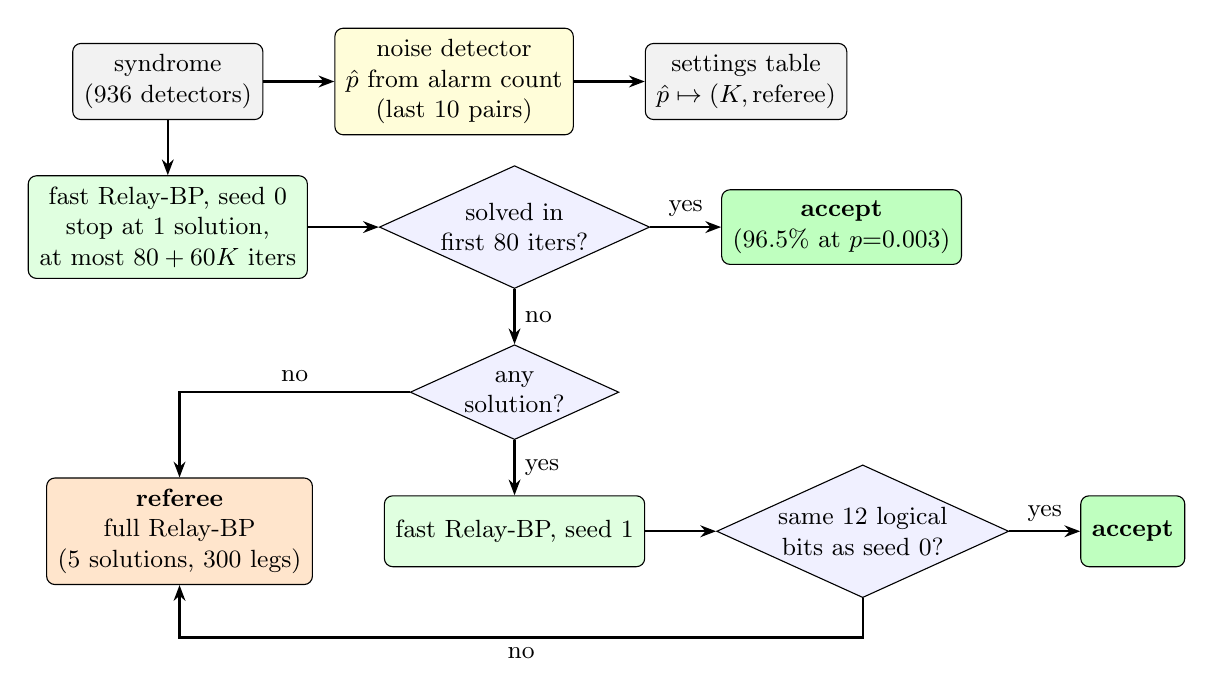
\begin{tikzpicture}[node distance=7mm and 9mm, font=\small,
  box/.style={draw, rounded corners=3pt, align=center, minimum height=9mm, inner sep=4pt, fill=#1},
  box/.default=white,
  dec/.style={draw, diamond, aspect=2.2, align=center, inner sep=1pt, fill=blue!6},
  arr/.style={-{Stealth[length=2mm]}, thick}]
  \node[box=gray!10] (in) {syndrome\\(936 detectors)};
  \node[box=yellow!15, right=of in] (est) {noise detector\\$\hat p$ from alarm count\\(last 10 pairs)};
  \node[box=gray!10, right=of est] (tab) {settings table\\$\hat p \mapsto (K, \text{referee})$};
  \node[box=green!12, below=of in] (s0) {fast Relay-BP, seed 0\\stop at 1 solution,\\at most $80+60K$ iters};
  \node[dec, right=of s0] (q1) {solved in\\first 80 iters?};
  \node[box=green!25, right=of q1] (acc1) {\textbf{accept}\\(96.5\% at $p{=}0.003$)};
  \node[dec, below=of q1] (q0) {any\\solution?};
  \node[box=green!12, below=of q0] (s1) {fast Relay-BP, seed 1};
  \node[dec, right=of s1] (q2) {same 12 logical\\bits as seed 0?};
  \node[box=green!25, right=of q2] (acc2) {\textbf{accept}};
  \node[box=orange!20, left=of s1] (ref) {\textbf{referee}\\full Relay-BP\\(5 solutions, 300 legs)};
  \draw[arr] (in) -- (est); \draw[arr] (est) -- (tab);
  \draw[arr] (in) -- (s0); \draw[arr] (s0) -- (q1);
  \draw[arr] (q1) -- node[above]{yes} (acc1);
  \draw[arr] (q1) -- node[right]{no} (q0);
  \draw[arr] (q0) -- node[right]{yes} (s1);
  \draw[arr] (q0) -| node[above, pos=0.25]{no} (ref);
  \draw[arr] (s1) -- (q2);
  \draw[arr] (q2) -- node[above]{yes} (acc2);
  \draw[arr] (q2.south) -- ++(0,-5mm) -| node[below, pos=0.25]{no} (ref.south);
\end{tikzpicture}
\caption{The decoder. The top row estimates the noise level and looks up the fast run's restart cap $K$ and which referee to use. Green boxes are cheap, the orange box is expensive, and the yellow box is the (optional) noise detector.
Seed 1 runs only when seed 0 needs more than its first leg (3\% of decodes at $p=0.003$). The referee runs on 0.6\% of decodes at $p=0.003$
and on about 21\% at $p=0.005$ (with $K=10$).}
\label{fig:flow}
\end{figure}

\paragraph{Why agreement works.} Relay-BP's later legs are randomised by their seed. A fast run that stops at its first
solution can be wrong. Two runs that share the deterministic first leg but use differently seeded later legs and still land on the \emph{same} logical class are
more likely to be right, and disagreement is a cheap, label-free warning sign. The gate rule itself has no trained parameters; its two settings ($K$ and the referee) were chosen on discovery data and
confirmed on separate seeds. The ``lean'' shortcuts follow from Relay-BP's structure:
\begin{itemize}
  \item \textbf{First-leg accept.} The first 80 iterations are deterministic, so seed 1 would reproduce seed 0 exactly.
        We verified 0 mismatches in about 34,000 shots, so the second run is skipped.
  \item \textbf{No solution $\Rightarrow$ referee.} If seed 0 finds nothing within its cap, a second fast run rarely
        helps, so the shot is escalated immediately.
\end{itemize}

\paragraph{Settings.} $K$ caps the fast run's restarts: it may use at most $80 + 60K$ iterations. The referee is
R5 (the kit's Relay-BP, which collects 5 solutions), R2 (2 solutions) or R1 (1 solution, 300 legs). The current table is
$K=10$ with R5 for $p \le 0.005$, $K=5$ with R2 at $p\approx0.0055$, and $K=5$ with R1 at $p\approx0.006$.
Section~\ref{sec:adaptive} explains how we chose it.

\paragraph{Implementation.} \texttt{experiments/gate.py} wraps the kit's \texttt{relay\_decoder} and exposes the same
\texttt{decode(syndrome)} interface. It is about 50 lines of Python, with no changes to the kit.

%=====================================================================
\section{How we tested}\label{sec:method}

Failures are rare (tens per 10,000 shots at $p=0.003$), so small runs mislead easily. Three of our own early
``findings'' disappeared on fresh data. We adopted the following rules and kept to them:
\begin{enumerate}
  \item \textbf{Same shots for every decoder.} Every decoder sees exactly the same sampled syndromes, and the decoder order
        is randomised per shot, so neither one benefits from a warm cache.
  \item \textbf{Pre-registration.} Before every confirmation run we wrote down the settings, sample sizes, seeds and pass/fail rules in
        \texttt{discussion/05}, \texttt{09}, \texttt{12}, \texttt{14} and \texttt{15}. Discovery and confirmation use
        disjoint seeds.
  \item \textbf{Accuracy verdict.} Pairs where exactly one decoder fails are ``discordant''. A one-sided 99.2\%
        Clopper--Pearson bound on the gate's share of discordant pairs gives an upper bound on the failure ratio
        gate/Relay-BP. \textbf{PASS} if the bound is $<1.2$, \textbf{FAIL} if the gate has more than 1.2$\times$ the failures,
        \textbf{INCONCLUSIVE} otherwise. The FAIL rule uses the observed counts, so with very few discordant pairs it is a weak signal. The 99.2\% level is a Bonferroni correction over six noise levels.
  \item \textbf{Latency verdict.} Paired bootstrap (2,000 resamples) 95\% upper bounds of the mean, p90 and p99 time
        ratios. \textbf{PASS} only if all three are below 1.
  \item \textbf{Machine.} An Apple-silicon Mac with 8 worker processes. Ratios are the claim. Absolute milliseconds are
        machine-specific, and 8 workers overstate speed-ups slightly (0.70$\times$ vs 0.79$\times$ single-worker at $p=0.004$).
\end{enumerate}

%=====================================================================
\section{Results}\label{sec:results}

\subsection{Headline: gate vs BP-OSD vs Relay-BP}

All numbers below come from fresh shots (seeds 5030--5050, and 6030 for the large run) decoded by all decoders. The gate uses
alarm-count routing and the revised settings table.

\begin{table}[H]
\centering\small
\begin{tabular}{lrrrrrrr}
\toprule
 & & \multicolumn{3}{c}{failed pairs} & \multicolumn{3}{c}{mean time per pair (ms)}\\
\cmidrule(lr){3-5}\cmidrule(lr){6-8}
$p$ & pairs & BP-OSD & Relay-BP & gate & BP-OSD & Relay-BP & gate\\
\midrule
0.003 & 10{,}000 & 55 & 5 & 7 & 94 & 57 & 22\\
0.003 & 100{,}000 & --- & 74 & 86 & --- & 77 & 30\\
0.004 & 6{,}000 & 336 & 55 & 53 & 282 & 262 & 191\\
0.005 & 3{,}000 & 726 & 262 & 262 & 578 & 1335 & 1164\\
\bottomrule
\end{tabular}
\caption{Failed X/Z pairs and mean decoding time (one X plus one Z shot). In the 100k run the gate was compared with Relay-BP only.}
\label{tab:headline}
\end{table}

\begin{figure}[H]
\centering
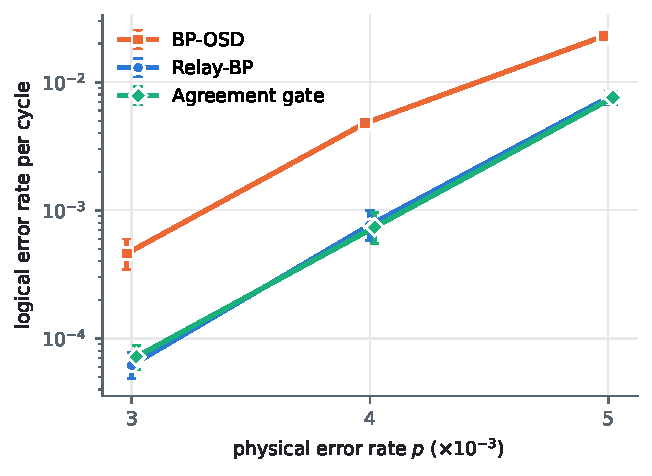
\includegraphics[width=0.56\textwidth]{ler_vs_p.pdf}
\caption{Logical error rate per cycle with 95\% intervals. The gate (green) lies on top of Relay-BP (blue) and is
3--8$\times$ below BP-OSD (orange). At $p=0.003$ the Relay-BP and gate points use the 100,000-pair run. Our Relay-BP value there
($6.2\times10^{-5}$) matches the authors' published $6.0\times10^{-5}$.}
\label{fig:ler}
\end{figure}

\begin{figure}[H]
\centering
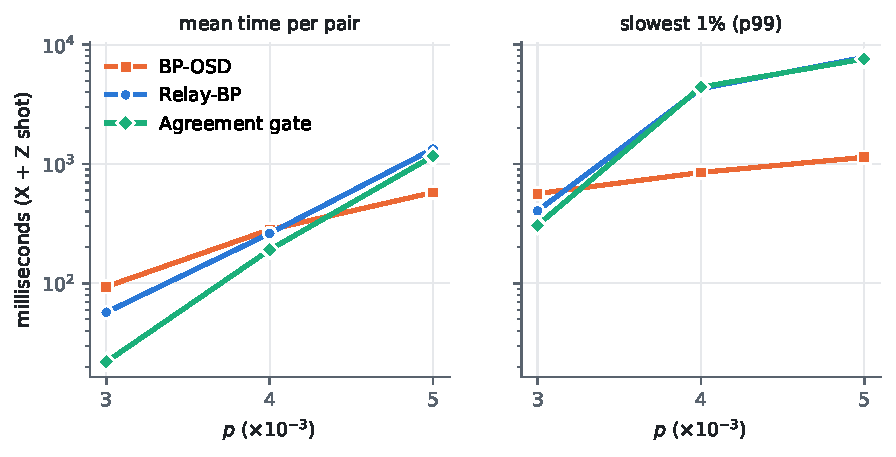
\includegraphics[width=0.85\textwidth]{latency_vs_p.pdf}
\caption{Decoding time. Left: the gate has the lowest mean time at $p=0.003$ and $0.004$, but at $0.005$ BP-OSD's fixed-cost
algorithm is fastest on average. Right: the slowest 1\% of shots. Relay-BP and the gate share a long tail
(seconds) that BP-OSD does not have.}
\label{fig:latency}
\end{figure}

\begin{table}[H]
\centering\small
\begin{tabular}{llllll}
\toprule
$p$ & fails (gate/RBP) & accuracy (bound) & mean & p99 & latency\\
\midrule
0.003 (100k) & 86 vs 74 & INCONCL.\ (1.46) & 0.39$\times$ & 0.73$\times$ & \textbf{PASS}\\
0.004 & 53 vs 55 & INCONCL.\ (1.29) & 0.73$\times$ & 1.03$\times$ & FAIL (p99)\\
0.005 & 262 vs 262 & \textbf{PASS} (1.11) & 0.87$\times$ & 0.97$\times$ & FAIL (p90 1.01$\times$)\\
\bottomrule
\end{tabular}
\caption{Pre-registered verdicts for the gate against Relay-BP (RBP). Time columns are gate/Relay-BP ratios. The 10k-pair run at $p=0.003$ gave 7 vs 5
(3 vs 1 discordant), which counts as FAIL under the observed-count rule, although 4 discordant pairs carry little information. The 100k run supersedes it.}
\label{tab:verdicts}
\end{table}

\paragraph{Reading the results.}
\begin{itemize}
  \item \textbf{Against BP-OSD} the gate is far more accurate at every noise level. It is faster on average at $p\le0.004$
        (0.23$\times$ and 0.68$\times$) and slower at $p=0.005$ (2.0$\times$). Its p99 is 5--7$\times$ worse at $p\ge0.004$. That tail
        comes from Relay-BP itself, not from the gate.
  \item \textbf{Against Relay-BP} the gate shows no significant difference in logical error rate and is faster on average
        everywhere: 2.6$\times$ at $p=0.003$, 1.4$\times$ at 0.004 and 1.15$\times$ at 0.005. Its tail is better at $p=0.003$ and roughly equal at $0.004$--$0.005$. At $p=0.003$ the best estimate is about $+16\%$ failures (86 vs 74), but the interval also includes no
        difference.
\end{itemize}

\subsection{Where the time goes}

\begin{figure}[H]
\centering
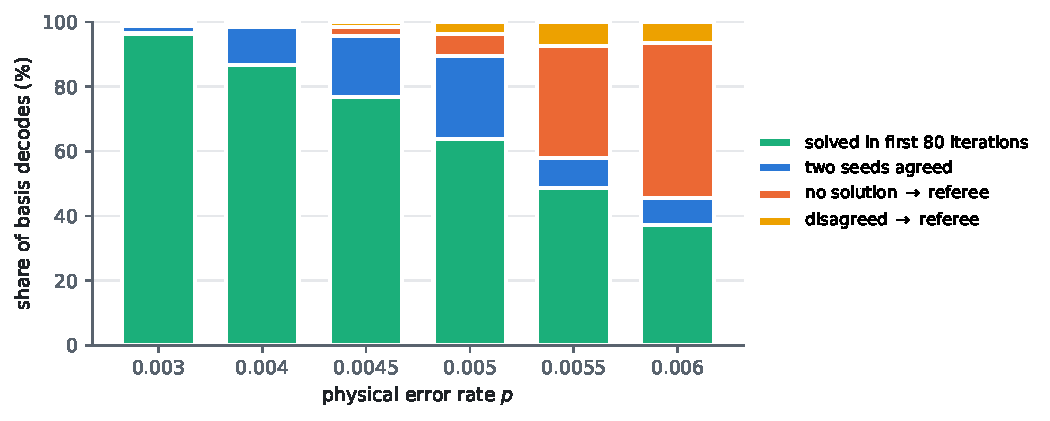
\includegraphics[width=0.8\textwidth]{gate_paths.pdf}
\caption{Path taken by each basis decode in the stage-2 confirmation runs ($K=50$ at $p=0.004$--$0.005$, $K=5$ elsewhere). At low noise almost every shot is solved in
the deterministic first 80 iterations and accepted immediately, which is why the gate is fast. As noise rises, more shots
reach the referee and the saving shrinks.}
\label{fig:paths}
\end{figure}

\subsection{Choosing settings by noise level}\label{sec:adaptive}

We tried 12 settings ($K\in\{5,10,20,50\}\times$ referee $\in\{$R5, R2, R1$\}$) at six noise levels on 24,500
discovery pairs. Capped runs were derived from the uncapped ones. Figure~\ref{fig:discovery} shows the trade-off.

\begin{figure}[H]
\centering
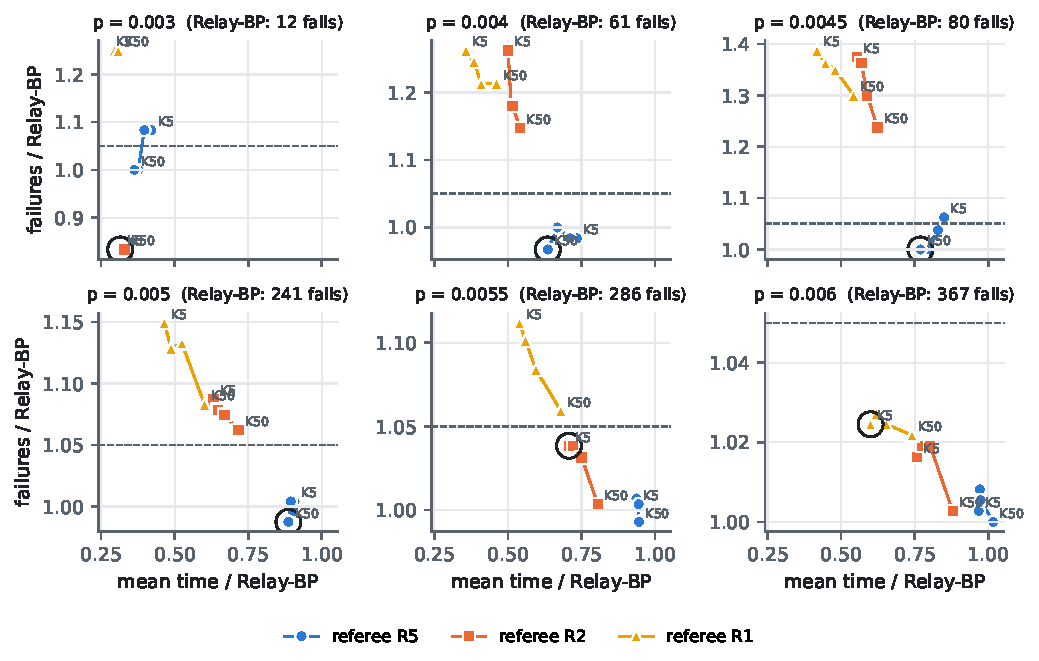
\includegraphics[width=0.95\textwidth]{discovery.pdf}
\caption{Stage-1 discovery: failures and mean time relative to Relay-BP for each setting. The dashed line is the 1.05
accuracy limit used for selection, and the circle is the setting chosen. Cheap referees (orange, yellow) cost 15--39\% extra
failures at $p=0.004$--$0.005$ but almost nothing at $p\ge0.0055$, where escalated shots usually fail whatever
the referee does.}
\label{fig:discovery}
\end{figure}

The stage-2 confirmation on fresh seeds taught three lessons:
\begin{itemize}
  \item \textbf{R2 at $p=0.003$ was a fluke.} Discovery picked it on 10 vs 12 failures. On fresh shots it gave 9 vs 2, and 6 of the 7 extra failures came
        from the R2 referee.
  \item \textbf{Large $K$ hurts the tail.} With $K=50$ the slowest 1\% were 14--16\% slower than Relay-BP, because the fast run
        burns up to 3,080 iterations before escalating. Lowering $K$ to 10 cut this to about 3\% (Table~\ref{tab:verdicts}).
  \item \textbf{$p=0.003$ is underpowered at 10k pairs.} Relay-BP alone gave 2, 14 and 7 failures in three such runs.
\end{itemize}

\subsection{The noise detector}

The team's design is: \emph{``when there is an alarm, the ML model detects the noise level and applies its effect''}.
We tested whether the noise level can be read from the alarms, and whether ML beats a simple count.

\begin{figure}[H]
\centering
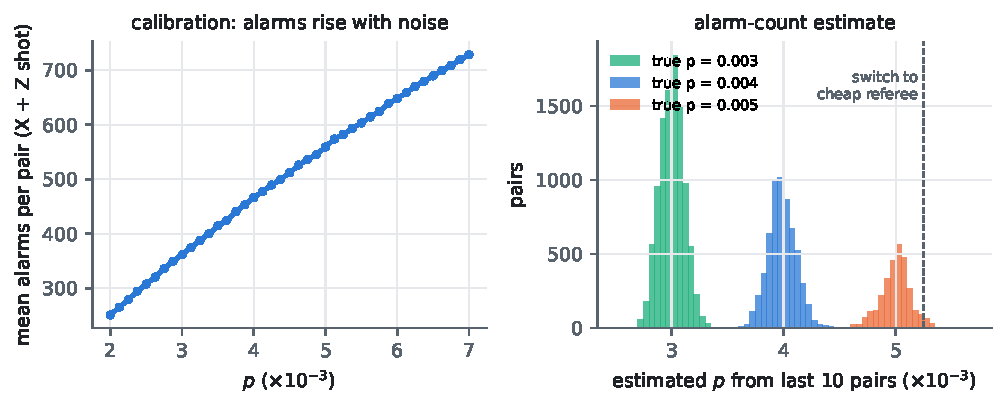
\includegraphics[width=0.9\textwidth]{noise_detector.pdf}
\caption{Left: the mean number of alarms rises smoothly with $p$, so the count is a natural estimator. Right: estimates
from the last 10 pairs on fresh shots. The three challenge noise levels separate cleanly. Only the 0.0053 boundary, where the
table switches to a cheap referee, matters for routing.}
\label{fig:noise}
\end{figure}

\begin{table}[H]
\centering\small
\begin{tabular}{lrrrr}
\toprule
estimator & 1 shot & last 10 & last 100 & cost per estimate\\
\midrule
alarm count + calibration curve & 6--9\% & 2--3\% & $\sim$0.8\% & $\sim$1\,$\mu$s\\
MLP (32, 16), alarm counts per cycle & 6--8\% & 2--3\% & 0.8--2.9\% & $\sim$70\,$\mu$s\\
ridge regression & 7--8\% & 2--4\% & 1--4\% & $\sim$60\,$\mu$s\\
\bottomrule
\end{tabular}
\caption{Mean relative error of the estimated $p$ on fresh shots ($p=0.003$--$0.006$). Training used 61,500 pairs at 41 noise levels.}
\end{table}

\begin{itemize}
  \item \textbf{Routing works.} In a stream whose noise changes every 300 pairs, count-based routing gave 203 failed pairs vs 207 for
        perfect knowledge of $p$, at the same time (0.67$\times$ Relay-BP).
  \item \textbf{ML adds nothing here.} On the 6,333-pair subset the MLP chose the same settings as the count on 100\%, 100\% and 97.3\% of pairs, with identical
        results. Under the kit's uniform noise model the total alarm count appears to carry nearly all the information about $p$.
  \item \textbf{Bias direction matters.} With the current table, over-estimating $p$ sends shots to cheap referees, and a
        $+10\%$ bias cost 11--18\% extra failures. The safe error is to under-estimate.
\end{itemize}

\subsection{Where the gate loses accuracy}

\begin{figure}[H]
\centering
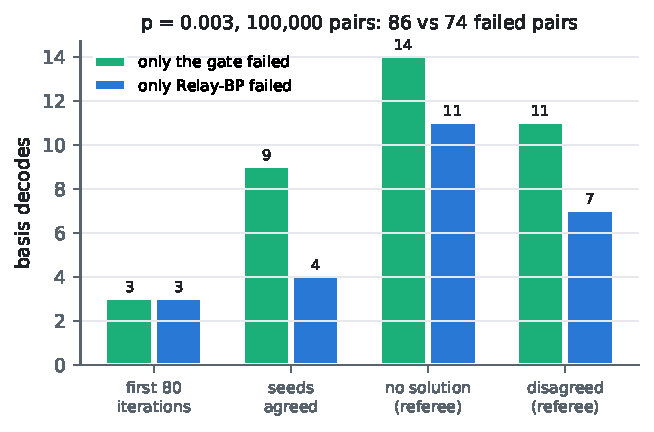
\includegraphics[width=0.6\textwidth]{p0003_discordance.pdf}
\caption{Discordant basis decodes in the 100,000-pair run at $p=0.003$, by gate path. The clearest excess is on the
``seeds agreed'' path (9 vs 4): both fast runs agree on a wrong logical class that the full Relay-BP, which compares 5 solutions, avoids.
These shots are the natural target for a learned per-shot check.}
\label{fig:disc}
\end{figure}

\subsection{A learned hard-shot spotter (tested, negative)}\label{sec:hardshot}
Following Figure~\ref{fig:disc}, we tested the ML component we had recommended: a classifier that looks at a syndrome
\emph{before} decoding and sends predicted-hard shots straight to the referee, skipping fast runs that would be wasted.
A wrong prediction can only cost time. The design was agreed with GPT and Gemini (\texttt{discussion/19}).
\begin{itemize}
  \item \textbf{Ceiling first.} Even a perfect spotter improves the mean by only 3--7 points. It moves the p99 ratio at $p=0.004$ from
        1.03 to 0.99 and the p90 ratio at $p=0.005$ from 1.01 to 0.97.
  \item \textbf{Models.} Logistic regression and gradient-boosted trees on microsecond syndrome features (alarm counts per cycle,
        other-basis alarms, adjacent alarm pairs, isolated alarms, repeats on the same check, and the noise estimate). The simple rule to beat is
        ``skip if the alarm count is high''. We trained on 50\% of the discovery shots, chose thresholds on 20\% and evaluated on the last 30\%,
        charging the measured inference cost (2\,$\mu$s for the rule, 112\,$\mu$s for logistic regression) to every decode.
  \item \textbf{Result.} The models separate shots the gate will escalate only moderately (AUC 0.69--0.74, about the same as the
        alarm count). Skipping an easy shot costs a full referee decode, so every policy, the simple rule included, chose to skip
        almost nothing, and held-out results equalled the plain gate. As agreed in advance, we stopped without a fresh-seed confirmation.
\end{itemize}
\emph{Lesson:} pre-decode syndrome summaries moderately predict escalation, but not well enough to pay for misrouted shots.
The more promising place for ML is in-flight: deciding after the first 80-iteration leg, from the decoder's own state,
whether to escalate early.

%=====================================================================
\section{Resources}\label{sec:resources}

\begin{itemize}
  \item \textbf{Decoder runs per basis decode.} At $p=0.003$: 1 fast run on 96.5\% of decodes, 2 on 2.9\%, and the
        referee on 0.6\%. At $p=0.005$: solved in the first leg on 64\%, and the referee on about 21\% with $K=10$ (20.6\% in discovery; Figure~\ref{fig:paths} shows the $K=50$ runs).
  \item \textbf{Iterations.} A first-leg accept uses at most 80 BP iterations. The fast run is capped at $80+60K = 680$ iterations ($K=10$).
        The referee is the unchanged kit Relay-BP.
  \item \textbf{Memory.} Three Relay-BP decoder objects per basis (two fast seeds and the referee). The noise detector is a 24-number feature vector
        and a lookup table, or a 2-layer MLP with about 2,100 weights.
  \item \textbf{Compute.} One CPU core per decode, and no GPU. All results were produced on a single laptop: roughly 4--5 hours of
        decoding for the experiments in this report.
\end{itemize}

%=====================================================================
\section{Lessons Learned and Limitations}

Developing an ML-assisted, multi-tiered decoding architecture for a high-distance bivariate bicycle code yielded several practical insights into quantum error correction pipelines, the mechanics of statistical consensus, and experimental methodology.

\subsection{Lessons Learned}

\subsubsection{Algorithmic Consensus Over Learned Classifiers}
Our most prominent finding was that learned acceptance gates (logistic regression and gradient-boosted trees on BP diagnostics) underperformed when tasked with accepting or escalating individual shots. Syndrome decoding on high-connectivity quantum codes operates under strict topological constraints where marginal probabilities do not trivially indicate coset correctness. Learned filters trained on internal belief propagation features produced unacceptable false-positive rates, yielding 5 excess logical failures at $p = 0.004$. In contrast, the zero-parameter Agreement Gate leveraged the stochastic nature of the perturbation process: requiring two runs with differently seeded later legs to arrive at identical 12-bit logical projections effectively suppressed logical errors without requiring threshold tuning.

\subsubsection{Physical Sufficiency of Aggregate Error Statistics}
Under spatially uniform, depolarizing circuit noise, spatial and temporal structures in detector firings provide negligible predictive value regarding overall error intensity. Complex feature embeddings (24 spatiotemporal check bins) mapped through a small neural network yielded no estimation advantage over a direct, scalar detector alarm count, which executed in $1\ \mu\text{s}$ with an error of $2\text{--}3\%$. In the absence of localized noise anomalies or anisotropic hardware defects, a simple alarm count appears to carry nearly all the information needed for online decoder scheduling.

\subsubsection{Asymmetry of Routing Thresholds}
In multi-tier systems, the penalties associated with threshold misclassification are highly asymmetric. Under-estimating physical noise defaults the system to conservative, highly capable decoders ($\text{R5}$), incurring a bounded latency overhead while preserving fidelity. Over-estimating physical noise by as little as $+10\%$, however, triggers aggressive truncation and routes complex syndromes to low-capability referees ($\text{R2}$, $\text{R1}$), resulting in an immediate $11\text{--}18\%$ surge in logical failures. Consequently, operational schedulers must incorporate deliberate downward conservatism.

\subsubsection{The Tyranny of the Latency Tail}
Accelerating the average case does not guarantee a performant quantum decoder. Cascaded decoders that execute sequentially (fast leg $\to$ verification leg $\to$ referee) inherently suffer from additive worst-case latencies on difficult syndromes. The lean agreement gate reduced mean execution time by up to $64\%$, but the first verified version made p99 latency $13\text{--}30\%$ worse at $p \ge 0.004$, because a long fast run was followed by the referee. Capping the fast run at $K=10$ restarts cut the p99 excess to about $3\%$ at $p=0.004$ (and $0.97\times$ at $p=0.005$, where p90 then failed by $1\%$); at $p=0.003$ the tail is $0.73\times$ Relay-BP's.

\subsubsection{Sample Sizing and Statistical Power in Low-Noise Regimes}
Benchmarking decoders at low logical error rates requires substantial sample sizes to avoid statistical noise. At $p = 0.003$, independent 10,000-shot evaluations of the identical baseline decoder yielded variance spanning 2 to 14 failures. Even an expanded trial of 100,000 pairs (86 gate failures vs.\ 74 baseline failures) proved statistically inconclusive under rigorous Bonferroni-corrected Clopper-Pearson bounds. Resolving a 20\% difference at $p=0.003$ needs well over $10^5$ pairs.

\subsubsection{Collaborative Multi-Agent Verification}
The structured interaction among three independent AI architectures (Claude, GPT, Gemini) served as an effective mechanism for error detection and experimental hygiene. Conceptual oversights, such as Gemini's low-weight acceptance threshold, an early claim that the gate was more accurate than Relay-BP, and the choice of the R2 referee at low noise, were systematically challenged and resolved through automated empirical falsification.

\subsection{Limitations}

Several limitations qualify the conclusions of this study:
\begin{itemize}
    \item \textit{Simulated Depolarizing Noise}: The benchmark evaluates circuit-level Pauli depolarizing noise simulated via Stim. Physical hardware implementations exhibit leakage, non-Markovian phase drift, cross-talk, and spatially inhomogeneous gate fidelities, which are not captured in uniform depolarizing models.
    \item \textit{Absence of Erasure Channels}: Although heralded qubit loss represents an active area of investigation for neutral-atom architectures, the evaluation harness provided no mechanism to inject or herald erasures.
    \item \textit{Sequential Execution Bottlenecks}: The prototype is orchestrated in Python and each decode runs on one core. Verification legs and referee fallbacks are invoked serially, forcing worst-case execution latency to equal the sum, rather than the maximum, of all stages.
    \item \textit{Hardware Platform Specifics}: Latency profiles were collected on a single 10-core Apple Silicon architecture utilizing 8 parallel workers. While relative execution ratios provide a normalized comparison, absolute millisecond latencies reflect the specific memory bus, cache hierarchy, and single-thread IPC of this platform. Multi-worker execution slightly inflated apparent speedups ($0.70\times$ mean runtime vs.\ $0.79\times$ in single-worker controlled environments).
    \item \textit{Discovery-Sample Overfitting}: Parameters governing the noise-adaptive table were tuned against discovery partitions. The failure of configuration $K5/\text{R2}$ during confirmation highlights the risk of overfitting discrete execution parameters to finite statistical samples.
\end{itemize}

%=====================================================================
\section{Where we are now}\label{sec:status}

\begin{table}[H]
\centering\small
\begin{tabular}{p{0.33\textwidth}p{0.6\textwidth}}
\toprule
Deliverable & Status\\
\midrule
LER sweep at $p=0.003, 0.004, 0.005$ & Done; Figure~\ref{fig:ler}, Table~\ref{tab:headline}\\
Latency vs BP-OSD and Relay-BP & Done; Figure~\ref{fig:latency}, Table~\ref{tab:verdicts}\\
Resources & Section~\ref{sec:resources}\\
GitHub repository & \href{https://github.com/ephan04/heisenbugsqc}{ephan04/heisenbugsqc}, branch \texttt{noise-adaptive-gate}\\
Plot and presentation & Figures in \texttt{report/figures}; slides to be made from this report\\
ML component & Noise detector and hard-shot spotter built and tested; neither beat a simple alarm-count rule (honest negative results)\\
Loss / heralding bonus & Not attempted (the kit does not simulate loss)\\
\bottomrule
\end{tabular}
\end{table}

\paragraph{Claim we can defend.} \emph{On the same simulated shots, the agreement-gated decoder makes 3--8$\times$ fewer
logical errors than BP-OSD. Its logical error rate shows no significant difference from Relay-BP's (non-inferiority shown at $p=0.005$), and it needs
13--61\% less mean decoding time. Its tail latency is better at $p=0.003$ and about equal at $p=0.004$--$0.005$.}

\paragraph{Claims we cannot make.} We cannot claim the gate is more accurate than Relay-BP, that it is non-inferior at $p=0.003$--$0.004$, that it improves tail latency at $p\ge0.004$,
or that either ML component (noise detector, hard-shot spotter) outperforms counting alarms.

%=====================================================================
\section{Next steps}\label{sec:next}
\begin{enumerate}
  \item \textbf{In-flight ML escalation.} The pre-decode spotter (Section~\ref{sec:hardshot}) did not pay off. The next ML candidate reads
        the decoder's state after the first 80-iteration leg (for example, unsatisfied checks and how they evolve) and decides whether to escalate
        early. This needs instrumenting Relay-BP. Checking agreed-but-wrong shots (Figure~\ref{fig:disc}) needs far more examples than we have.
  \item \textbf{Parallel stages.} Run seed 0, seed 1 and the referee concurrently on separate cores, so that latency becomes the
        maximum of the stages instead of their sum. This is the most direct fix for the tail.
  \item \textbf{Harder noise.} Use non-uniform or drifting noise (for example measurement errors $\ne$ gate errors), where a learned
        detector could beat a single count.
  \item \textbf{Loss and heralding.} Add \texttt{HERALDED\_ERASE} to the circuits and feed erasure locations to the priors.
  \item \textbf{Generality.} Repeat on \texttt{bb72}/\texttt{bb90}/\texttt{bb108} with \texttt{make\_circuit.py}.
\end{enumerate}

%=====================================================================
\appendix
\section{Reproducing the results}
\begin{small}
\begin{verbatim}
uv venv --python 3.12 .venv
uv pip install -r challenge-1-ml-decoder-kit/requirements.txt matplotlib
# headline comparison (BP-OSD, Relay-BP, gate with alarm-count and MLP routing)
python experiments/bposd_compare.py --p 0.004 --shots 6000 --seed 5040 \
       --out data/compare_p0.004.npz
python experiments/bposd_compare_report.py data/compare_p*.npz
# 100k pairs at p = 0.003
python experiments/adaptive_confirm.py --p 0.003 --shots 100000 --seed 6030 \
       --table results/revised_p0.003.json --out data/large_p0.003.npz
# settings discovery and confirmation, noise detector, figures
python experiments/adaptive_collect.py ...
python experiments/adaptive_select.py data/adapt_p*.npz
python experiments/noise_ml.py
python experiments/report_figures.py
\end{verbatim}
\end{small}
All raw data are in \texttt{data/} and every summary is in \texttt{results/}. The full three-AI discussion, including
each pre-registration, is in \texttt{discussion/}, and every prompt is listed in \texttt{PROMPTS.md}.

\section{How this report was written}
The team lead directed the work through Claude Code. Claude ran the experiments, wrote the code and integrated this report.
GPT (via \texttt{codex}) drafted Sections~1--2 and Gemini (via \texttt{agy}) drafted Section~3 and the lessons section, both from a
shared fact sheet (\texttt{discussion/17\_report\_brief.md}). Both then fact-checked the assembled draft. Every number traces
to a file in \texttt{results/}.

\end{document}
